% AI-assisted shared draft prepared at Ayushi's request on 25 October 2026.
% Assigned reviewer: Guruprasad Simimath. Live screenshots captured for the report on 25 October 2026.
\subsection{Frontend and user workflow}
\label{subsec:frontend_workflow}

The frontend is a custom HTML, CSS and JavaScript application connected to the RAG pipeline through a local Python HTTP server. It displays answers, calculations, source references and evidence limitations. Health checks support the connection indicator, while the document library endpoint provides the report list~\cite{fintraceRuntime2026}.

Users can ask a question directly or select optional bank and financial year filters. A bank or year named in the question takes precedence; filters supply missing context. Users do not need to classify their request as a lookup, definition or explanation. The interface accepts up to 2,000 characters and retains up to eight successful responses in the current browser tab. This history is not a persistent account or an archive available on other devices.

Financial labels remain visible beside figures. Supported comparisons show their calculation workings, and numbered references lead to extracted evidence and the original PDF page. Responses can be copied or downloaded as JSON, a structured format for inspecting the result. These controls let an analyst examine how an answer was produced rather than relying on its wording alone.

Partial answers and evidence limitations are displayed explicitly. A quotation selected from a report is distinguished from a generated explanation because a relevant passage may not establish a requested ranking or cause. Figures~\ref{fig:frontend_profit} and~\ref{fig:frontend_comparison} illustrate two live examples already used during development. They demonstrate the interface rather than provide a new accuracy or latency assessment.

\begin{figure}[!htbp]
\centering
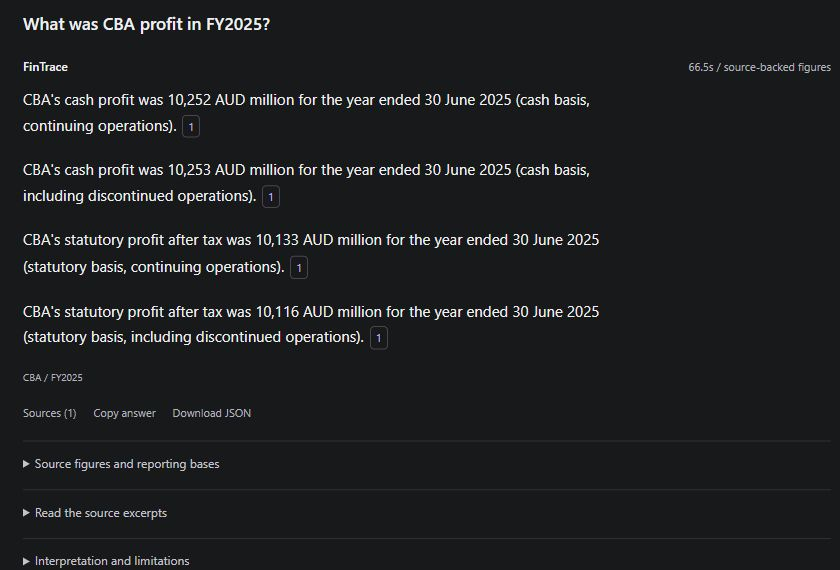
\includegraphics[width=0.98\linewidth]{frontend_profit.png}
\caption[Frontend: labelled profit alternatives]{Live interface response to ``What was CBA profit in FY2025?'' Four figures linked to source cells distinguish cash/statutory basis and continuing/total operations. The numbered references identify CBA's FY2025 Profit Announcement, PDF page 18~\cite{fintraceCBA2025}.}
\label{fig:frontend_profit}
\end{figure}

\begin{figure}[!htbp]
\centering
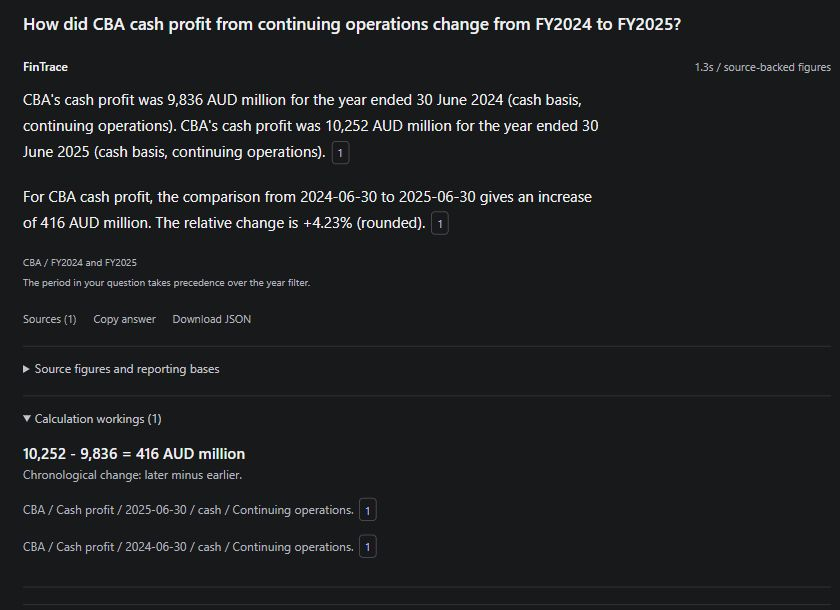
\includegraphics[width=0.98\linewidth]{frontend_comparison.png}
\caption[Frontend: comparison and calculation workings]{Live interface comparison of CBA continuing cash profit from FY2024 to FY2025. The expanded workings show AUD~10,252 million minus AUD~9,836 million, giving AUD~416 million; the answer reports approximately 4.23\% relative growth. Operand references lead to PDF page 18 of the FY2025 report. Screenshots are illustrative runs, not timing guarantees.}
\label{fig:frontend_comparison}
\end{figure}

The prototype runs locally for a single user. Its evidence, models and indexes require installation beyond cloning the repository. Model startup and competition for GPU resources can affect response time. Checks of interface state and server behaviour were recorded separately from financial answer assessment. Formal accessibility, multi-user load and analyst usability studies remain future work.
